\section{Simulation results}
This section is about the simulation results which were achieved.
First, these results are presented.
......
The simulation was performed in Sinalgo\footnote{http://www.disco.ethz.ch/projects/sinalgo/}.
Sinalgo is a simulation framework which can test and validate network algorithms and at the same time it offers a graphical view on the programmed processes as well as a fast batch mode.

There are two different simulation runs.
The first one calculated the Euclidean and hop spanning ratio of PDT and RMYS and the second one counted the messages which were needed to construct PDT, RMYS and the amount of messages needed by two hop beaconing.
1000 random connected graphs for each node density from 5 to 20 were used.
The numbers of nodes $n $ used for each density were calculated with the following formula:
\begin{equation*}
n =round( \frac{D_x \cdot D_y}{\pi \cdot R^2} \cdot density)
\end{equation*}
Hereby, $D_x=1000 $ and $D_y=1000 $ are the dimension of the simulation plane and $R = 100 $ is the unit disk radius.

\bigskip

The simulations are based on the following assumptions.
\begin{itemize}
\item All nodes are static meaning they cannot move.
\item All calculations are ordered into synchronous rounds. 
At the beginning a node receives all messages sent in the round before.
It follows a general calculation phase and at last a node can send messages.
\item Messages arrive instantaneously and cannot get lost.
Every message which was sent, arrives for sure in the round after it was sent.
\item There are no 4 nodes which are co-circular.
\item All graphs are connected.
\end{itemize}

Figure \ref{fig:RMYS_PDT_SpanningRatio} shows the measured spanning ratio of RMYS and PDT to the unit disk graph with respect to node density.
It is noticeable that both lines seem to be the same line.
For density $5 $ the ratio is approximately $1.30 $ and density 20 has approximately a spanning ratio of $1.38 $.
In between 5 and 20 the curve is increasing slightly and has no outliers.

Since both lines are almost identical it is possibly true that RMYS also has a constant spanning ratio which is a fractional amount greater than the proven spanning ratio of PDT (refer to \cite{Neumann2012} for the proven spanning ratio).

\begin{figure}[h!]
\centering
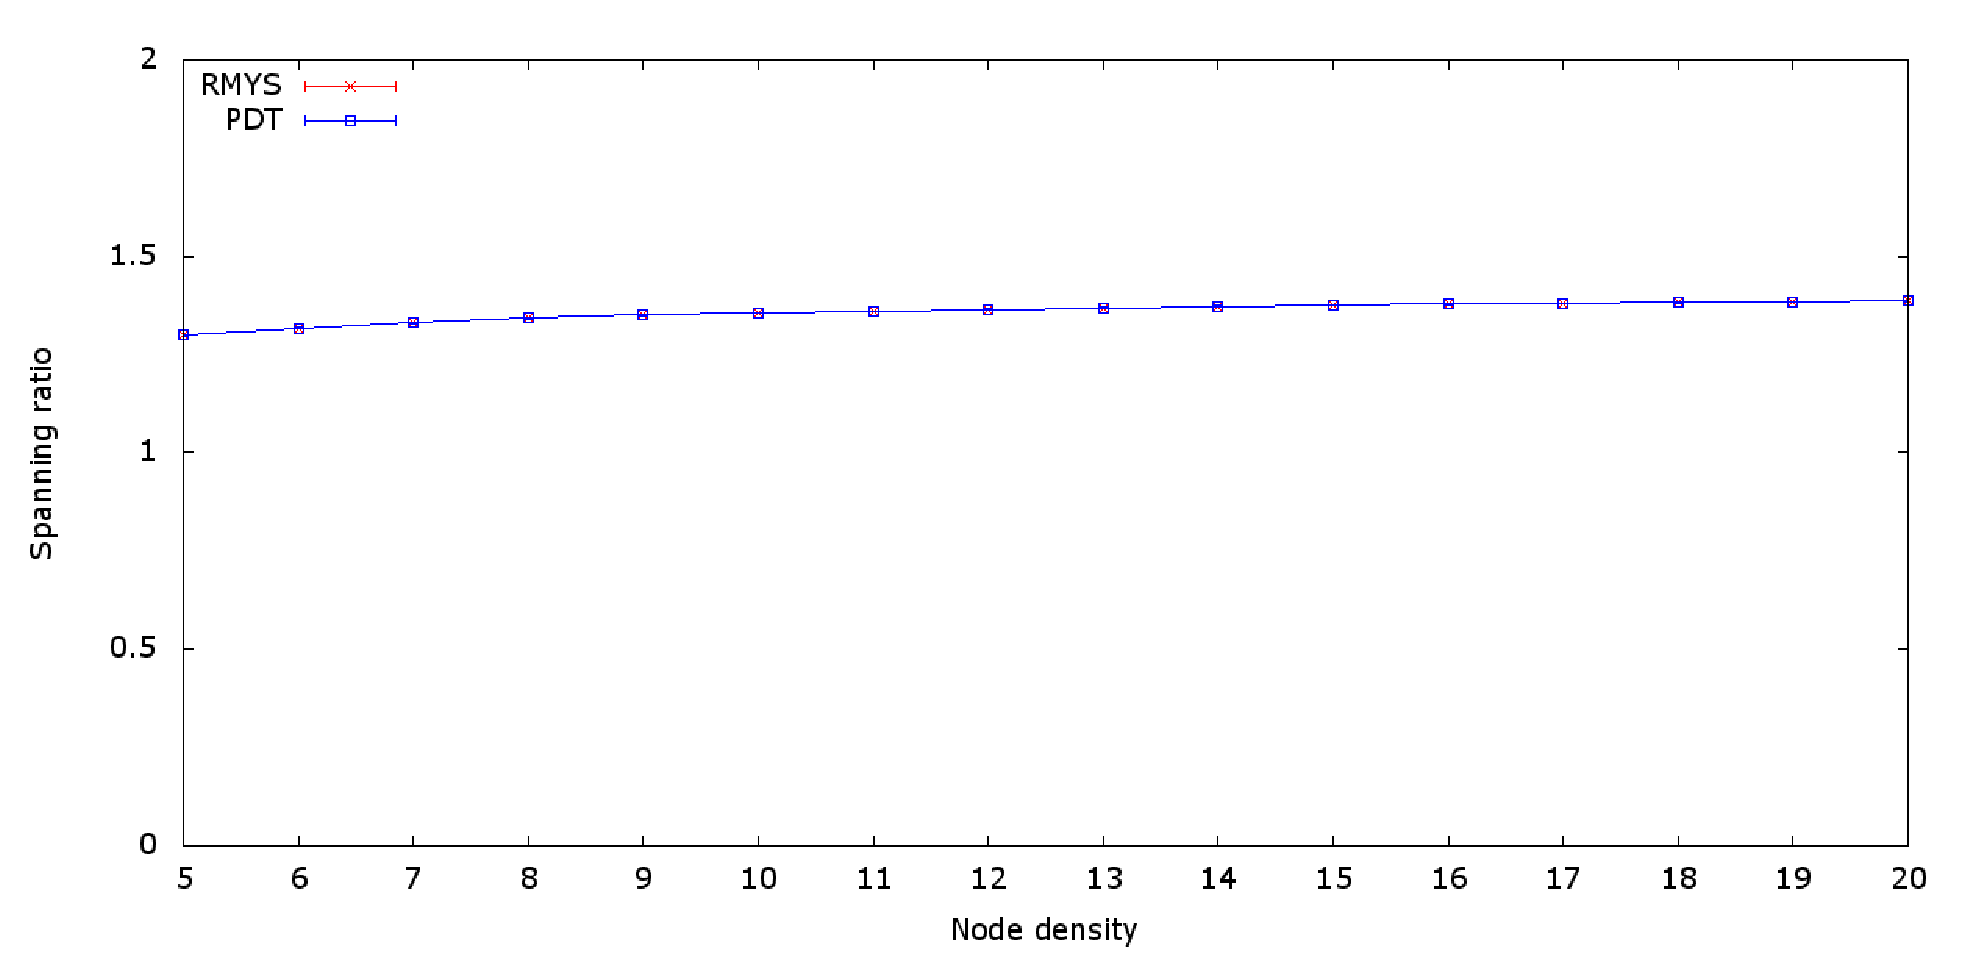
\includegraphics[width=1.0\linewidth]{eps/RMYS_PDT_SpanningRatio.eps}
\caption{Measured Euclidean spanning ratio of Reactive Modified Yao Step (RMYS) and Partial Delaunay Triangulation (PDT) with respect to the unit disk graph in context to the node density. 1000 Simulations per density.}
\label{fig:RMYS_PDT_SpanningRatio}
\end{figure}


Figure \ref{fig:RMYS_PDT_HopSpanningRatio} shows the measured hop spanning ratio of RMYS and PDT to the unit disk graph with respect to node density.
The measured values increase from $3 $ hops at density $5 $ to approximately $4.6 $ at density $20 $.

\begin{figure}[h!]
\centering
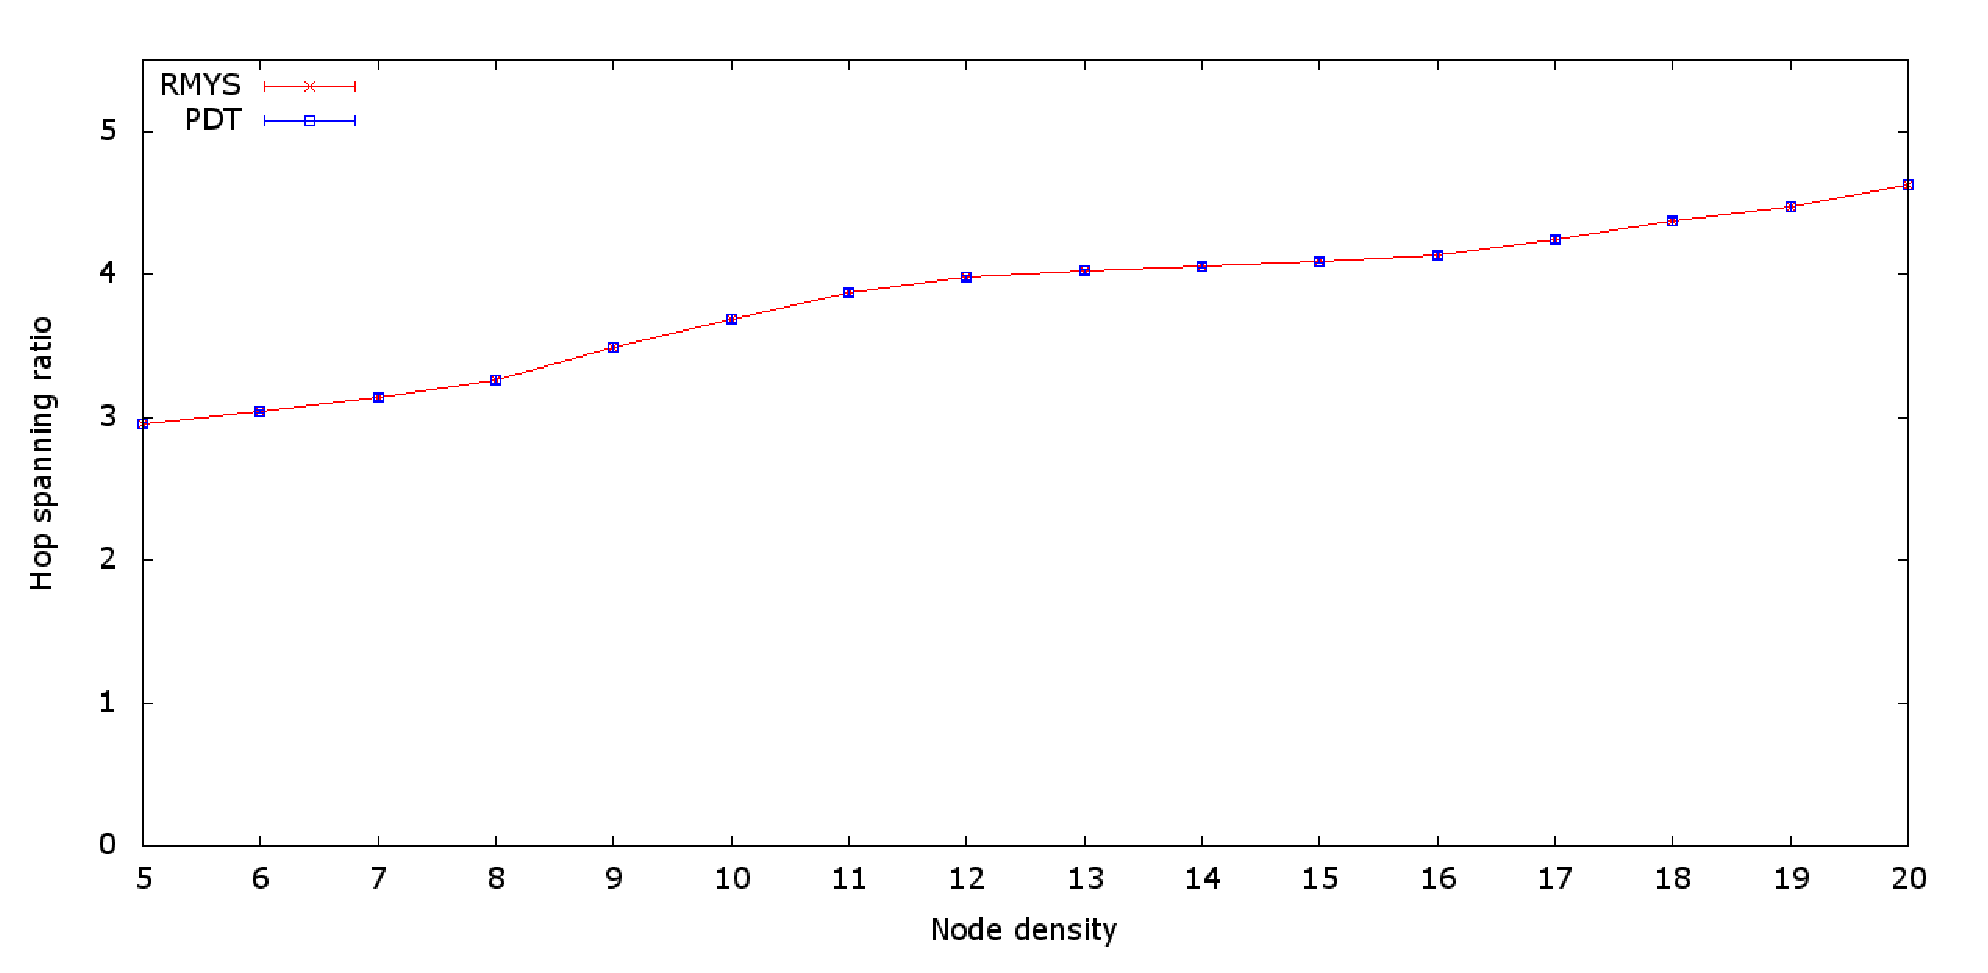
\includegraphics[width=1.0\linewidth]{eps/RMYS_PDT_HopSpanningRatio.eps}
\caption{Measured hop spanning ratio of Reactive Modified Yao Step (RMYS) and Partial Delaunay Triangulation (PDT) with respect to the unit disk graph in context to the node density. 1000 Simulations per density.}
\label{fig:RMYS_PDT_HopSpanningRatio}
\end{figure}



In figure \ref{fig:RMYS_PDT_Beaconing_Neighbors.eps} is the message consumption with respect to node density shown.
"PDT on neighbors" shows the amount of messages PDT uses to create the 2 hop PDT neighborhood of one random node within the graph borders and at least unit disk radius $R=100 $ away from the borders to ensure the correct node density.
In this example the amount of messages RMYS and PDT on neighbors uses are almost equal.
The messages used in 2 hop beaconing are much more.
Additionally, the increase from one density to another is greater than the increase in PDT and RMYS.
At density $5 $ beaconing uses almost twice as much messages as RMYS and at density $20 $ it uses almost tenth times as much messages as RMYS.
For reference, the amount of messages which PDT uses to create the 1 hop PDT neighborhood of the same node as above is shown.
Notice that PDT is message optimal (refer to \cite{Benter2013} for proof) in terms of only nodes which are actually PDT neighbors send messages.

\begin{figure}[h!]
\centering
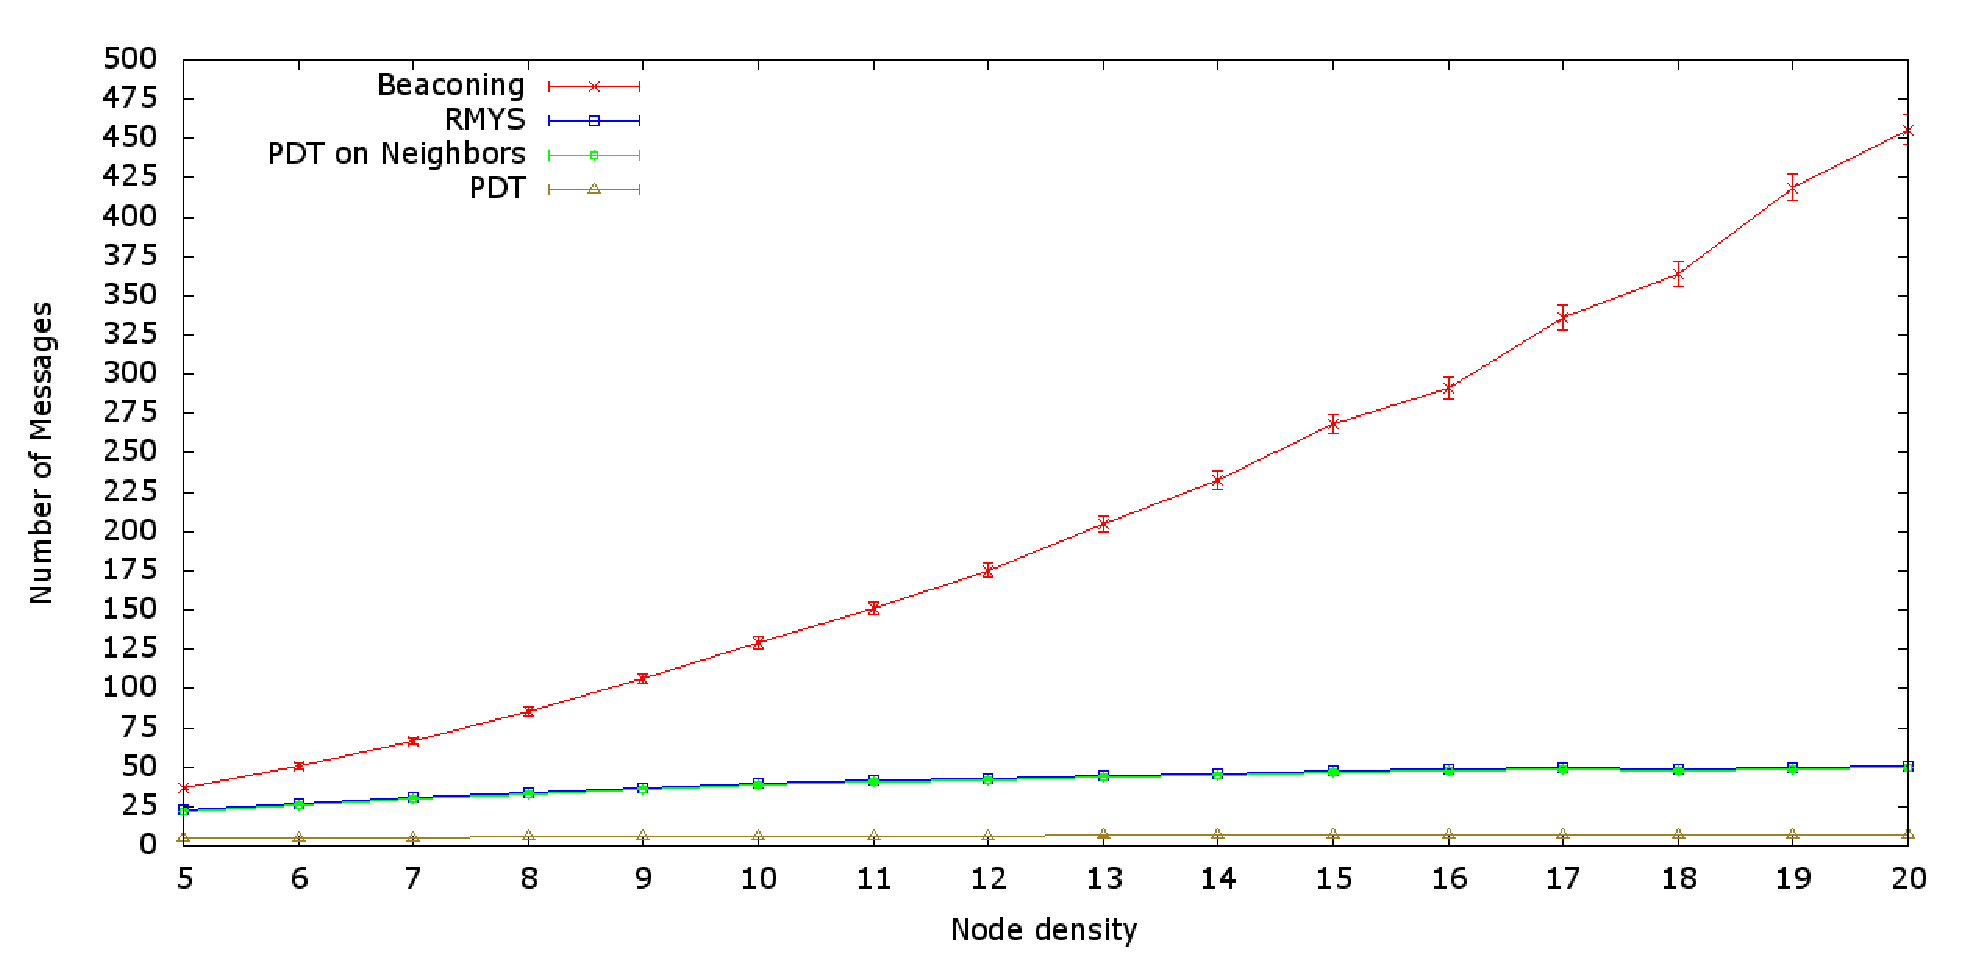
\includegraphics[width=1.0\linewidth]{eps/RMYS_PDT_Beaconing_Neighbors.eps}
\caption{This plot shows the needed messages to construct the RMYS-neighborhood on a given node with respect to the node density in a 2-hop beaconing approach (Beaconing) and in a reactive way (RMYS). Additionally, the messages rPDT uses to construct the PDT-neighborhood of a node (PDT) and its neighbors (PDT on Neighbors) are shown. 1000 Simulations per density.}
\label{fig:RMYS_PDT_Beaconing_Neighbors.eps}
\end{figure}

Figure \ref{fig:RMYS_PDT_Neighbors} shows the message consumption with respect to node density between RMYS and PDT on neighbors in order to notice the small differences.
In fact RMYS uses always one message more than PDT on neighbors.
For reference, the message consumption for PDT on one node is shown as well.

\begin{figure}[h!]
\centering
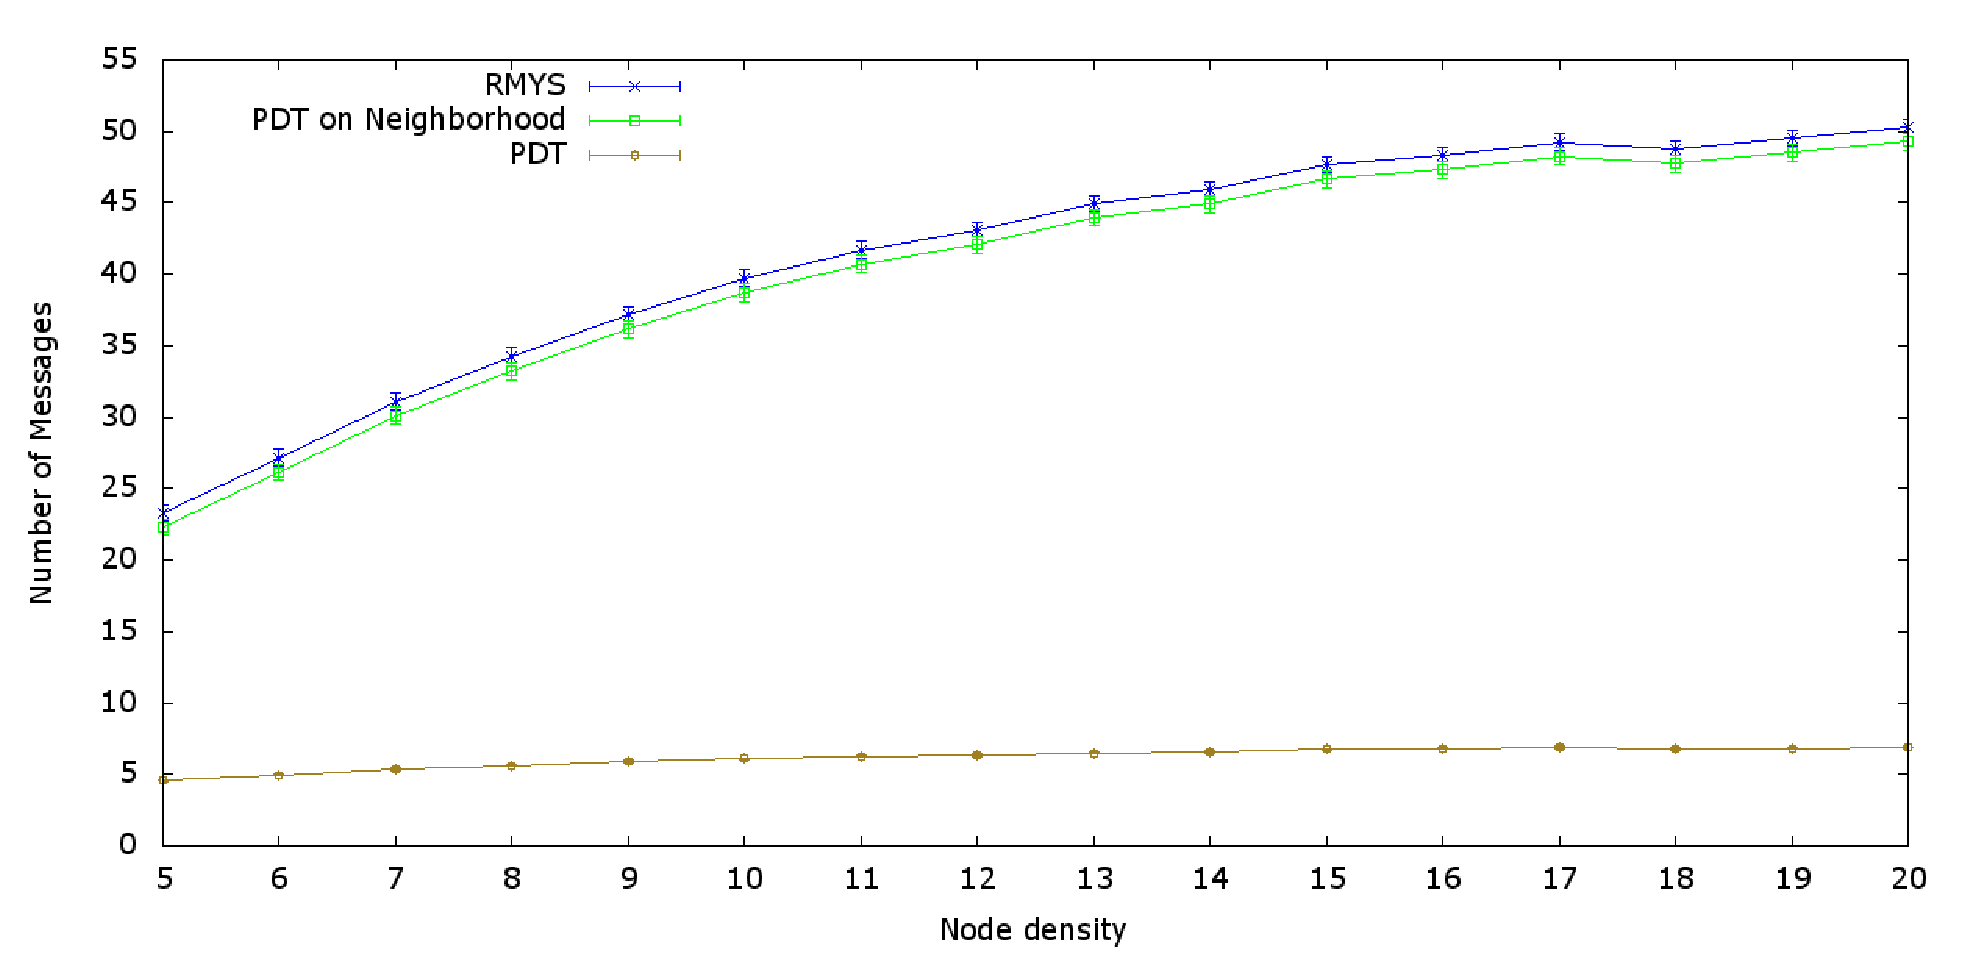
\includegraphics[width=1.0\linewidth]{eps/RMYS_PDT_Neighbors.eps}
\caption{The messages needed to construct the PDT-neighborhood of a node (PDT) and its neighbors (PDT on Neighbors) are shown. Additionally, the message usage of the RMYS neighborhood creation is visualized. 1000 Simulations per density.}
\label{fig:RMYS_PDT_Neighbors}
\end{figure}


Refer to figure \ref{fig:RMYS_PDT_avrNeighbors} to see the average and maximal neighbors of the RMYS and the PDT graph.
Density $5 $ leads to approximately $3.6 $ neighbors and almost $6 $ neighbors at density $20 $.
The maximal neighbors differ for both graphs from $6.89 $ at density $5 $ to approximately $10.35 $ for RMYS and $10.44 $ for PDT at density $20 $.
The differences of the maximal neighbors for RMYS and PDT at high densities is explained in REF.

\begin{figure}[h!]
\centering
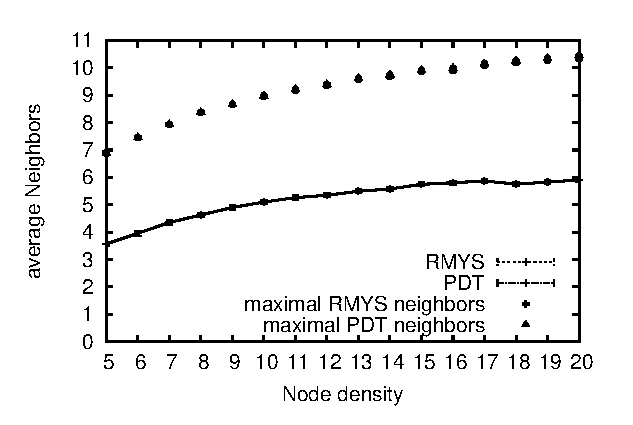
\includegraphics[width=1.0\linewidth]{eps/RMYS_PDT_avrNeighbors.eps}
\caption{Average and maximal Neighbors of Reactive Modified Yao Step (RMYS) and Partial Delaunay Triangulation (PDT) with respect to node density. 1000 Simulations per density.}
\label{fig:RMYS_PDT_avrNeighbors}
\end{figure}


Figure \ref{fig:RMYS_PDT_UDGNeighborsRatio} shows the amount of neighbors in the subgraphs RMYS and PDT of a random node divided by the amount of neighbors in the unit disk model of the same node.
A value of $1 $ corresponds to all unit disk neighbors are neighbors in the subgraph.
At density $5 $ approximately $0.8 $ percent of all unit disk neighbors are PDT and RMYS neighbors.
At density $20 $ this percentage dropped to $0.33 $.

\begin{figure}[h!]
\centering
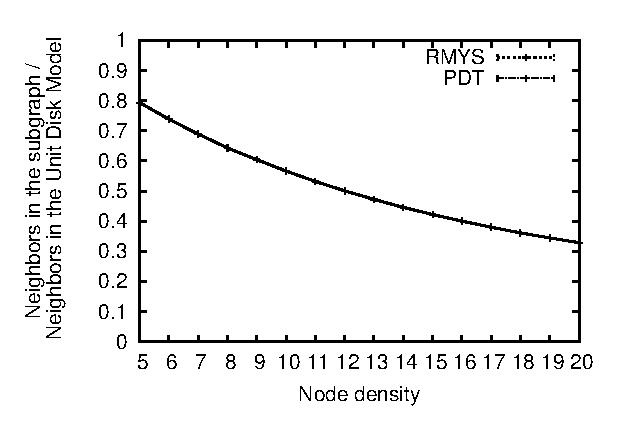
\includegraphics[width=1.0\linewidth]{eps/RMYS_PDT_UDGNeighborsRatio.eps}
\caption{The average neighbors for Reactive Modified Yao Step (RMYS) and Partial Delaunay Triangulation (PDT) divided by the average neighbors in the unit disk model are shown. 1000 Simulations per density.}
\label{fig:RMYS_PDT_UDGNeighborsRatio}
\end{figure}

\begin{figure}[h!]
\centering
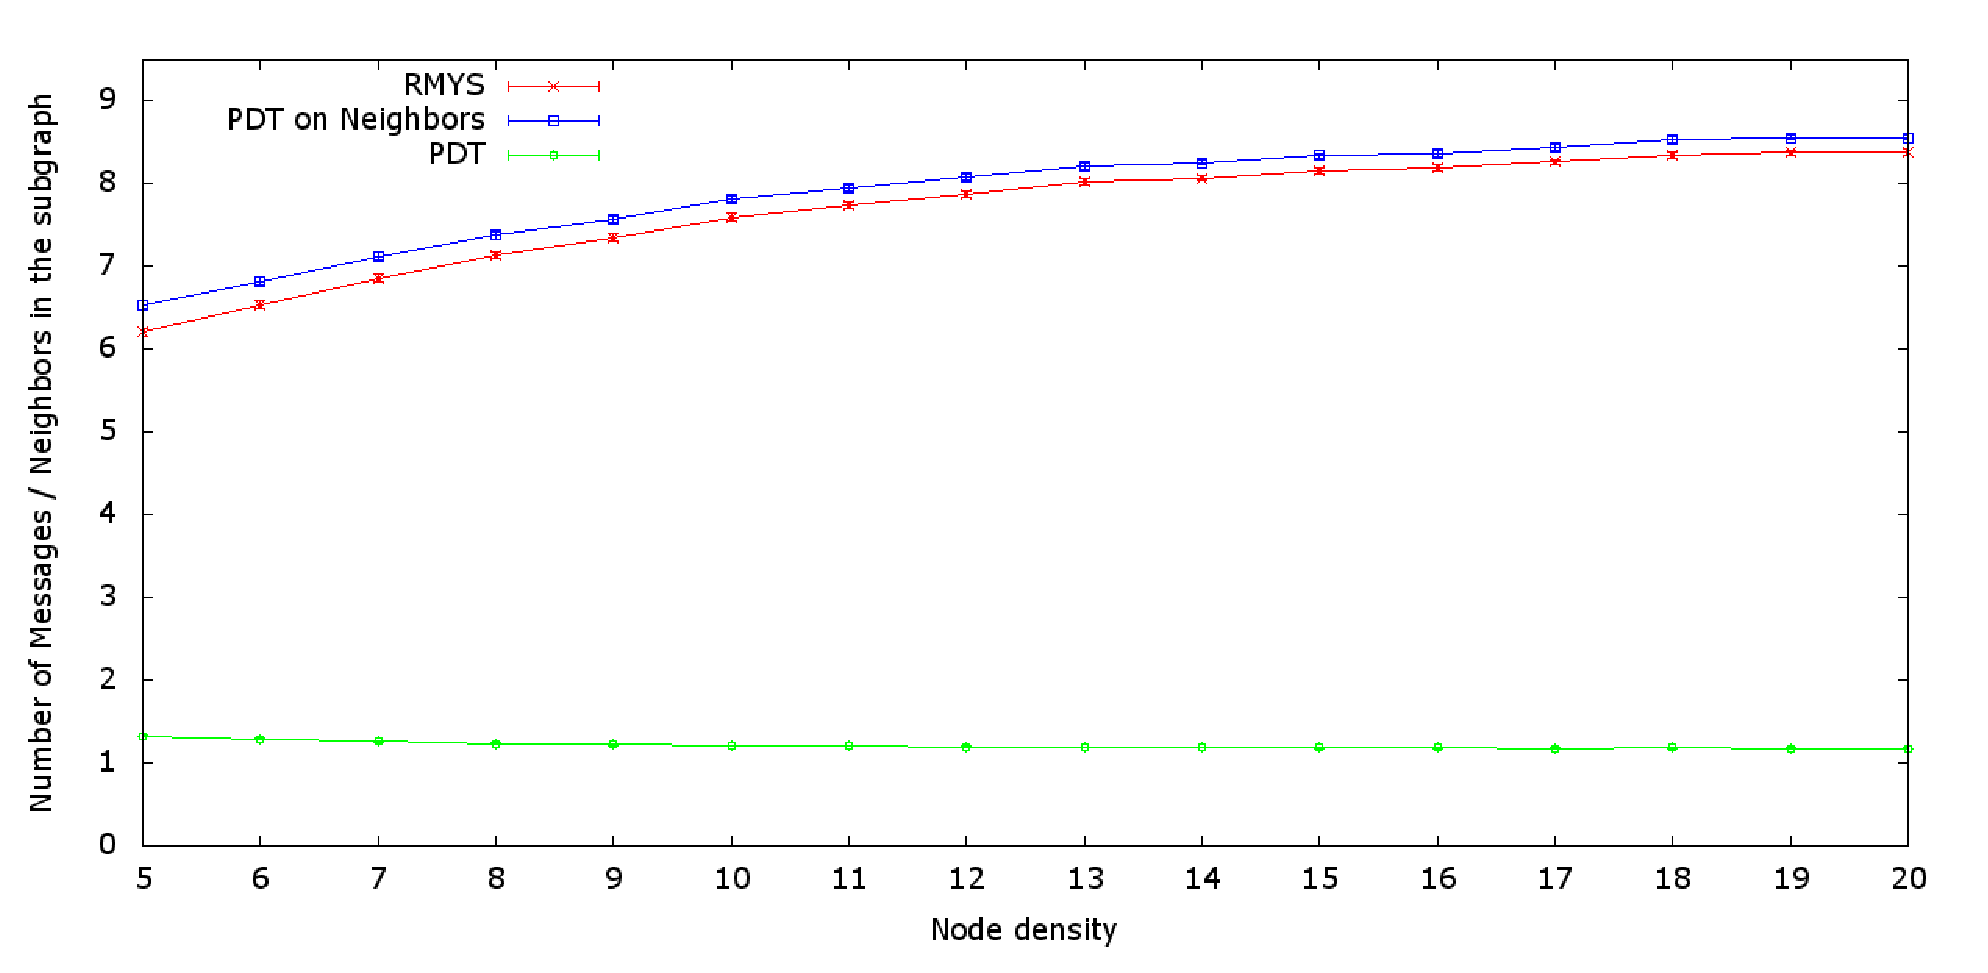
\includegraphics[width=1.0\linewidth]{eps/RMYS_PDT_MessagesPerNeighbors.eps}
\caption{The messages needed to construct the RMYS neighborhood (RMYS), the PDT neighborhood of a node (PDT) and its neighbors (PDT on Neighbors) divided by the actual neighbors in this subgraph are visualized. 1000 Simulations per density.}
\label{fig:RMYS_PDT_MessagesPerNeighbors}
\end{figure}

In Figure \ref{fig:RMYS_PDT_MessagesPerNeighbors} is the number of used messages by a topology control divided by the obtained neighbors in the specific subgraph visualized.
Here, $1 $ corresponds to for each neighbor in the subgraph $1 $ message was sent.
PDT uses not much more than this.
At density $5 $ PDT sends approximately $1.33$ and at density $20 $ approximately $1.18 $ messages per neighbor.
PDT on neighbors and RMYS send $6.2 $ and $6.5 $, respectively, messages per neighbor at density $5 $.
At density $20 $ PDT on neighbors uses $8.4 $ and RMYS $8.6 $ messages per neighbor.

\section{Discussion}
In the following the simulation results are interpreted and explained.
Additionally, 
There are two cases where RMYS does not select all neighbors of a node, even if the count of these neighbors is below the limit of $k=14 $.
Both cases are presented briefly in the following.
First, notice figure \ref{fig:RMYS_case_error_bidirectional}.
This figure contains two nodes $u $ and $v $ with one of their RMYS cones drawn.
The blue circles and the dotted line marked with $R $ symbolize the unit disk radius of both nodes.
The green circle proofs that $uv $ is a PDT edge.
Suppose that the red area contains a node $n $ and that any other cone of $v $ (not visualized) also contains one node.
If RMYS is executed on that example, $u $ selects $v $ in any case since it is the only node in that cone.
However, $v $ selects $n $ since it is closer to $v $ than $u $.
All other cones contain nodes as well and therefore no more edges are selected.
As a result of this behavior the edge $uv $ was selected from only one, namely $u $, of its endpoints and therefore, $v $ sends a protest message.

\begin{figure}[h!]
\centering
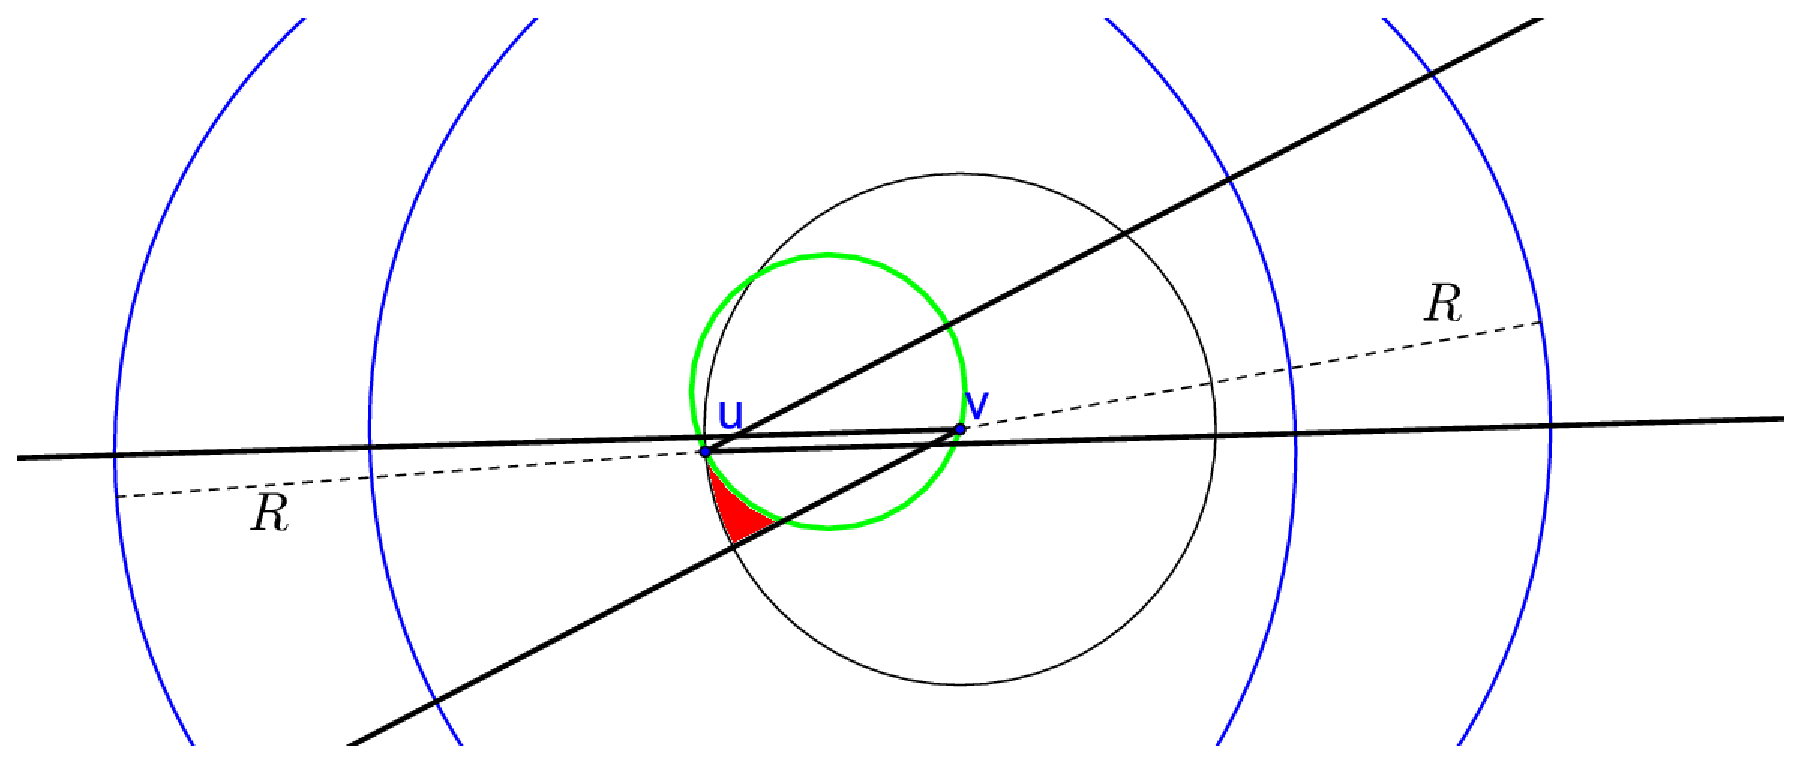
\includegraphics[width=1.0\linewidth]{eps/RMYS_case_error_bidirectional.eps}
\caption{Node $u $ and $v $ are drawn with a specific cone and blue unit disk circles with radius $R $. The green circle is the PDT circle for edge $uv $ and if the red area contains a point, $uv $ is no bidirectional RMYS edge.}
\label{fig:RMYS_case_error_bidirectional}
\end{figure}


\begin{figure}[h!]
\centering
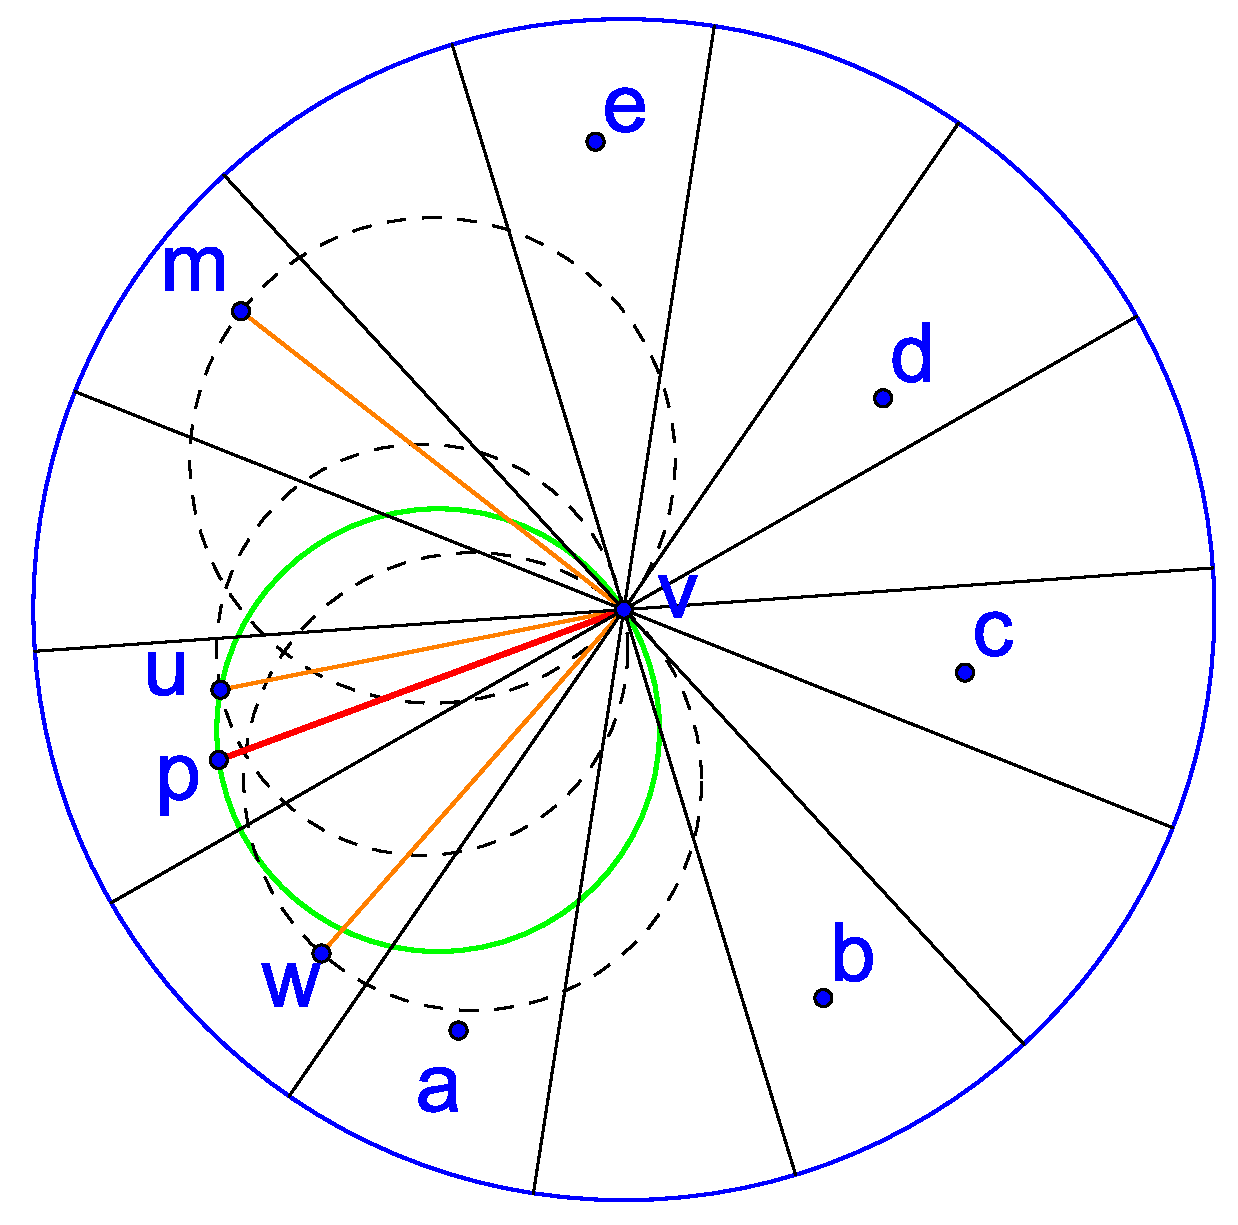
\includegraphics[width=0.7\linewidth]{eps/RMYS_case_one_cone_empty.eps}
\caption{An example graph with specific edges drawn which are incident on $v $. The blue circle symbolize the unit disk. The dotted circles are Gabriel circles and the green one proofs the existence of $uv $ and $pv $ in the PDT graph.}
\label{fig:RMYS_case_one_cone_empty}
\end{figure}

An example for the second case can be viewed in figure \ref{fig:RMYS_case_one_cone_empty}.
It shows a view on an example graph with all edges drawn which are incident on $v $.
In addition, the Gabriel circles of some nodes are visualized in a dotted way.
The green circle through $u $, $v $ and $p $ proofs that $vp $ is a PDT edge.
Note that nodes $a,b,c,d $ and $e $ are also PDT neighbors of $v $, even though their Gabriel circles and edges to $v $ are not drawn for simplicity of this figure.
RMYS executed on node $v $ leads to the selection of all edges incident on $v $ except $pv $.
First, all shortest edges per cone are selected which leads to the selection of $uv $ for the cone containing $u $ and $p $.
Since there is no sequence of empty cones which is longer than 1 only edges which are closest to the empty cones are considered and therefore, $pv $ is not being selected.
For this case to happen it is mandatory that there is no sequence of length longer than 1 or the edge is, possibly, being selected.
However, it is not needed that between nodes $a,b,c,d $ and $e $ is always one empty cone.
There can also be none.
This is a minimal example in terms of node usage.

In order to understand the small deviation of maximal neighbors at high densities between RMYS and PDT both above explained cases must be taken into account.
In addition, the maximal neighbors in figure \ref{fig:RMYS_PDT_avrNeighbors} were calculated over all nodes in a graph and the actual neighbors for the specific subgraphs were instead calculated for one random node per graph.
The small difference of less than $1 \% $ between both subgraphs and the fact that no node in the complete simulation has sent a protest message leads to the conclusion that with the parameter $k = 14 $ both above cases can be neglected.
However, both cases might be relevant for theoretical proofs concerning the spanning ratio or lowering the bound of $k = 14 $.



